\section{行程问题}

\title[第4讲\quad 行程问题]{第4讲\quad 行程问题} 
\author{}
\date{}

\begin{frame}
    \titlepage
\end{frame}

\setcounter{framecounter}{0}

\begin{frame}
    \stepcounter{framecounter}
    \frametitle{习题\theframecounter}
    \textit{一辆公共汽车和一辆小轿车同时从相距450千米的两地相向而行,公共汽车每小时行40千米,小轿车每小时行50千米,\underline{\hbox to 20mm{}}小时后两车第二次相距90千米 .} 
    % 6
\end{frame}

\begin{frame}
    \stepcounter{framecounter}
    \frametitle{习题\theframecounter}
    \textit{小文今天和朋友约定一起看 12:00 开场的电影,出门时,发现挂钟电池没电已经停止了,她把挂钟换好电池,但没来得及调整时间,出门前挂钟显示的时间是 9:25,小文赶到电影院时,电影刚好开场.电影结束后,小文立刻返回家中,发现挂钟显示的时间是 13:55,小文赶紧把它调成正确的时间15:45.如果小文从家到电影院和从电影院返回家中花的时间是一样的,那么,电影的时长是\underline{\hbox to 10mm{}}分钟.}
    \begin{figure}[H] 
        \centering
        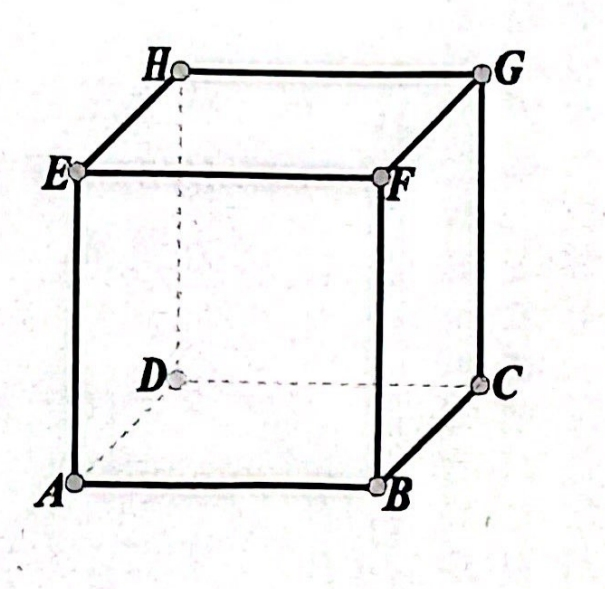
\includegraphics[width=0.2\textwidth]{./pics/Chapter_4/2.png}
    \end{figure}
    % 2022. 180
\end{frame}


\begin{frame}
    \stepcounter{framecounter}
    \frametitle{习题\theframecounter}
    \textit{一条圆形跑道长 600 米,因铺设水管,其中跑道上 AB 一段被挖开,形成一个大坑。AB的跑道长度为 150 米。 有一机器人放在跑道上循环行走, 前进的步长(跑道弧长)为 d米,可调整步长 d的大小,但调后不再改变,并且 d小于 600 米.请设计出两种(d 的不同长度)方案,使得机器人不断循环,并且永远不会落入坑里(碰到 A或 B也算落入坑里)每种方案包括:\\
    (1)步长d的值(不同方案的d的值)。\\
    (2)机器人的出发点。.}
    \begin{figure}[H] 
        \centering
        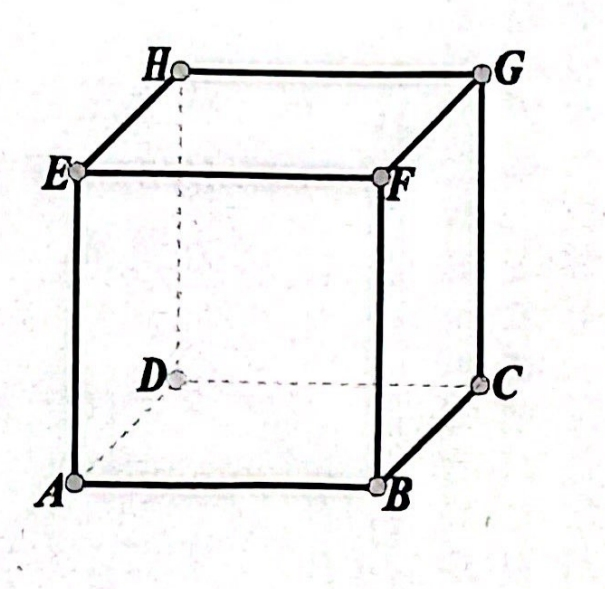
\includegraphics[width=0.2\textwidth]{./pics/Chapter_4/2.png}
    \end{figure}
    % 
\end{frame}


\begin{frame}
    \stepcounter{framecounter}
    \frametitle{习题\theframecounter}
    \textit{哥哥和弟弟两人同时从家出发去 2000米外的学校上学,哥哥每分钟走 60米,弟弟每分钟走 50 米,走了 10 分钟后,哥哥发现忘记带数学错题本,就以每分钟 100 米的速度跑回家,回到家后,哥哥用了2分钟找到了错题本,然后以每分钟 150 米的速度往学校跑.从哥哥第二次从家出发开始计算,经过\underline{\hbox to 10mm{}}分钟后,哥哥能追上弟弟.}
    \begin{figure}[H] 
        \centering
        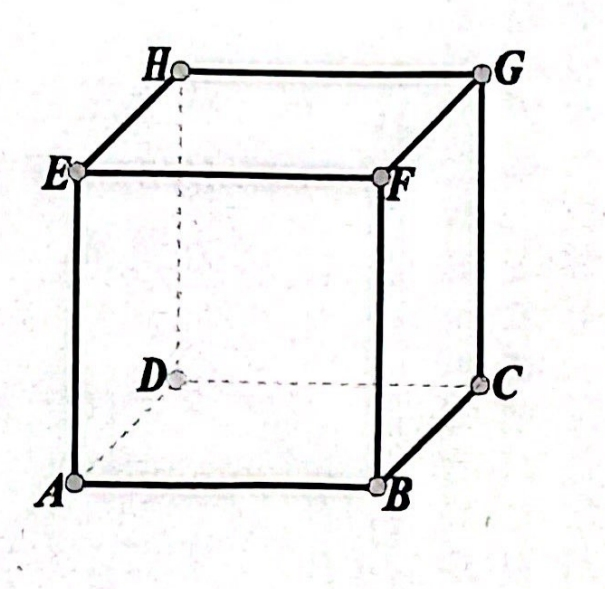
\includegraphics[width=0.2\textwidth]{./pics/Chapter_4/2.png}
    \end{figure}
    % 2020华, 9
\end{frame}

\begin{frame}
    \stepcounter{framecounter}
    \frametitle{习题\theframecounter}
    \textit{甲、乙两车分别从A,B两地同时出发,相向而行,3小时后相遇,甲掉头返回A地,乙继续前行.甲到达A地后掉头往B行驶,半小时后和乙相遇.那么乙从A到B共需\underline{\hbox to 10mm{}}小时.}
    % 2011华, 7.2
\end{frame}


\begin{frame}
    \stepcounter{framecounter}
    \frametitle{习题\theframecounter}
    \textit{甲、乙两车分别从A,B两地同时出发,相向而行,3小时后相遇,甲掉头返回A地,乙继续前行.甲到达A地后掉头往B行驶,半小时后和乙相遇.那么乙从A到B共需\underline{\hbox to 10mm{}}小时.}
    % 2011华, 7.2
\end{frame}

\begin{frame}
    \stepcounter{framecounter}
    \frametitle{习题\theframecounter}
    \textit{一个车队以4米/秒的速度缓慢通过一座长298米的大桥,共用115秒,已知每辆车长6米,相临两车间隔20米,则这个车队一共有 \underline{\hbox to 10mm{}} 辆车.}
    % 2012华, 7
\end{frame}


\begin{frame}
    \stepcounter{framecounter}
    \frametitle{习题\theframecounter}
    \textit{四百米比赛进入冲刺阶段,甲在乙前面30米,丙在丁后面60米,乙在丙前面20米.这时,跑在前面的两位同学相差 \underline{\hbox to 10mm{}} 米.}
    % 2012华, 10
\end{frame}

\begin{frame}
    \stepcounter{framecounter}
    \frametitle{习题\theframecounter}
    \textit{里山镇到省城的高速路全长189千米,途径县城.县城离里山镇54千米.早上8:30一辆客车从里山镇开往县城,9:15到达.停留15分钟后开往省城,午前11:00能够到达.另有一辆客车于当日早上9:00从省城径直开往里山镇.每小时行驶60千米.两车相遇时,省城开往里山镇的客车行驶了 \underline{\hbox to 10mm{}} 分钟.}
    % 2012华, 72
\end{frame}

\begin{frame}
    \stepcounter{framecounter}
    \frametitle{习题\theframecounter}
    \textit{一艘轮船,从上游A地开往下游B地,需要1小时,原路返程时,将船速提高到原来的2倍,也需要1小时.那么,如果游轮从A地出发时也采用2倍船速,需要  \underline{\hbox to 10mm{}} 分钟可以到达B地.}
    % 2014华, 36
\end{frame}

\begin{frame}
    \stepcounter{framecounter}
    \frametitle{习题\theframecounter}
    \textit{一条河上有A,B两个码头,A在上游,B在下游.甲、乙两人分别从A,B同时出发,划船相向而行,4小时后相遇.如果甲、乙两人分别从A,B同时出发,划船同向而行,乙16小时后追上甲.已知甲在静水中划船的速度为每小时6千米,则乙在静水中划船每小时行驶\underline{\hbox to 10mm{}}千米.}
    % 2015华, 10
\end{frame}

\begin{frame}
    \stepcounter{framecounter}
    \frametitle{习题\theframecounter}
    \textit{甲、乙两人在一条长120米的直路上来回跑,甲的速度是5米/秒,乙的速度是3米/秒,若他们同时从同一端出发跑了15分钟,则他们在这段时间内共迎面相遇 \underline{\hbox to 10mm{}} 次(端点除外).}
    % 2015华, 23
\end{frame}

\begin{frame}
    \stepcounter{framecounter}
    \frametitle{习题\theframecounter}
    \textit{甲、乙两车分别从A,B两地同时出发,相向匀速行进,在距A地 60 千米处相遇.相遇后,两车继续行进,分别到达B,A后,立即原路返回,在距B地50 千米处再次相遇.则A,B两地的路程是\underline{\hbox to 10mm{}}千米.}
    % 2016华, 130
\end{frame}

\begin{frame}
    \stepcounter{framecounter}
    \frametitle{习题\theframecounter}
    \textit{猎豹跑一步长为2米,狐狸跑一步长为1米.猎豹跑2步的时间狐狸跑3步.猎豹距离狐狸30米,则猎豹跑动\underline{\hbox to 10mm{}}米可追上狐狸.}
    % 2017华, 120
\end{frame}
